\subsubsection{RFID}
\label{subsubsec:Inbetriebnahme_RFID}

Beim RFID-Leser handelt es sich wie in Kapitel \ref{subsec:RFID} um das MFRC522 Evaluierungsboard (Breakout-Board). Dieses Kommuniziert über SPI mit einem gewünschten Controller. Die Pinbelegung dazu ist in Abbildung \ref{fig:MFRC522} zu sehen. Der grosse Vorteil dieses Evaluirungsboard ist es, dass es dazu eine Arduino Library gibt mit vielen Beispielen.

Um den Leser in Betrieb nehmen zu können, wurde dieser wie folgt angeschlossen:


\begin{itemize}
\item Vcc: An 3.3V vom ESP32
\item GND: An GND vom ESP32
\item SDA: An IO5 vom ESP32
\item SCK: An IO18 vom ESP32
\item MISO: AN IO19 vom ESP32
\item Reset: AN IO22 vom ESP32
\item MOSI: AN IO23 vom ESP32
\end{itemize}

\begin{figure}[h!]
\center
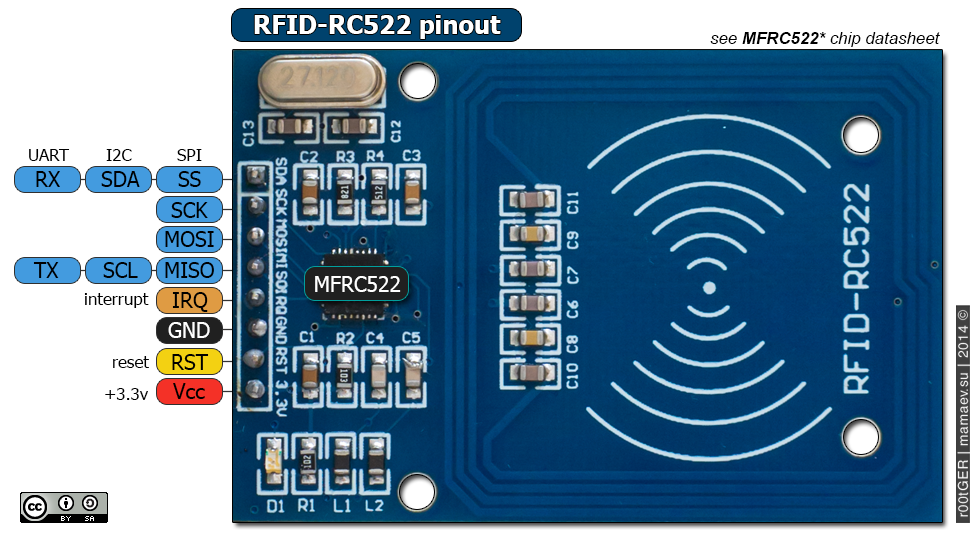
\includegraphics[width = 0.58\textwidth]{graphics/MFRC522}
\caption{Anschauungsbild MFRC522 Evaluierungsboard}
\label{fig:MFRC522}
\end{figure}

Diese Pinbelegung ist von der Arduino-Library gegeben und wird auch so bei der Cocktailmaschine eingesetzt, da es keinen Grund gibt diese direkt in der Library zu ändern. Lediglich die beiden Pin's \flqq SDA\frqq~und \flqq Reset\frqq~können flexibel festgelegt werden.

Um das Lesegerät in Betrieb nehmen zu können, wurde nach dem Anschliessen der Pin's Arduino IDE geöffnet. 




\todo{Quelle: https://www.heise.de/developer/imgs/06/2/0/1/4/1/0/3/RFID-RC522-pinout-5a5263ece3c12e96.png}

